
\begin{section}{Experimentación}
 No se comparó la simulación contra un fluido real bajo las mismas condiciones. Sin embargo la simulación parece reflejar correctamente el comportamiento de un fluido, como puede apreciarse en el \href{https://www.youtube.com/watch?v=D8JOELu8uAs}{grafico de velocidad}, o en el \href{https://www.youtube.com/watch?v=_JisfmOIEdU}{grafico del aspa} de las figuras \ref{fig:sim_hm_all} y \ref{fig:sim_vf_all}
~\\
\begin{figure*}
    \textbf{Grafico de la velocidad}\par\medskip

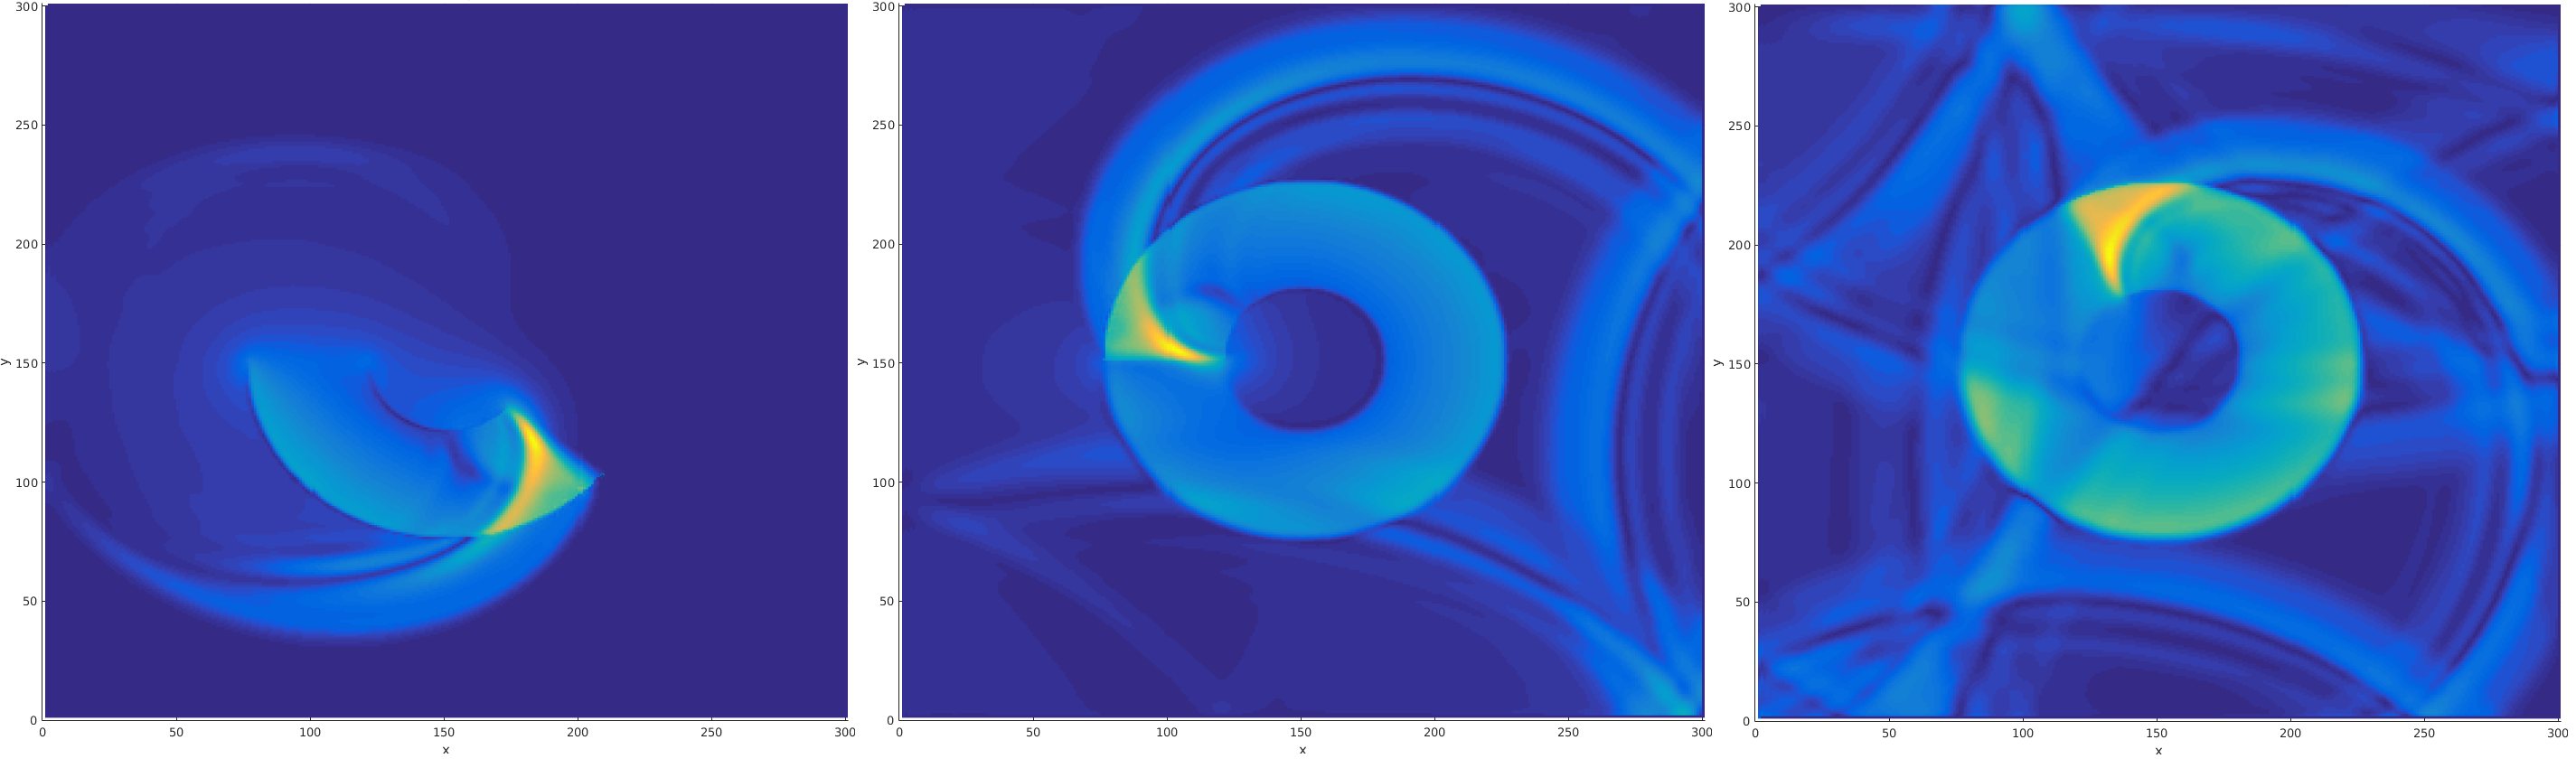
\includegraphics[width=\textwidth,height=4cm]{figures/sim_hm_all}
\caption{Estos mapas de calor muestran la evolución del fluido en el tiempo.}
\label{fig:sim_hm_all}
\end{figure*}

\begin{figure*}
    \textbf{Grafico del aspa}\par\medskip

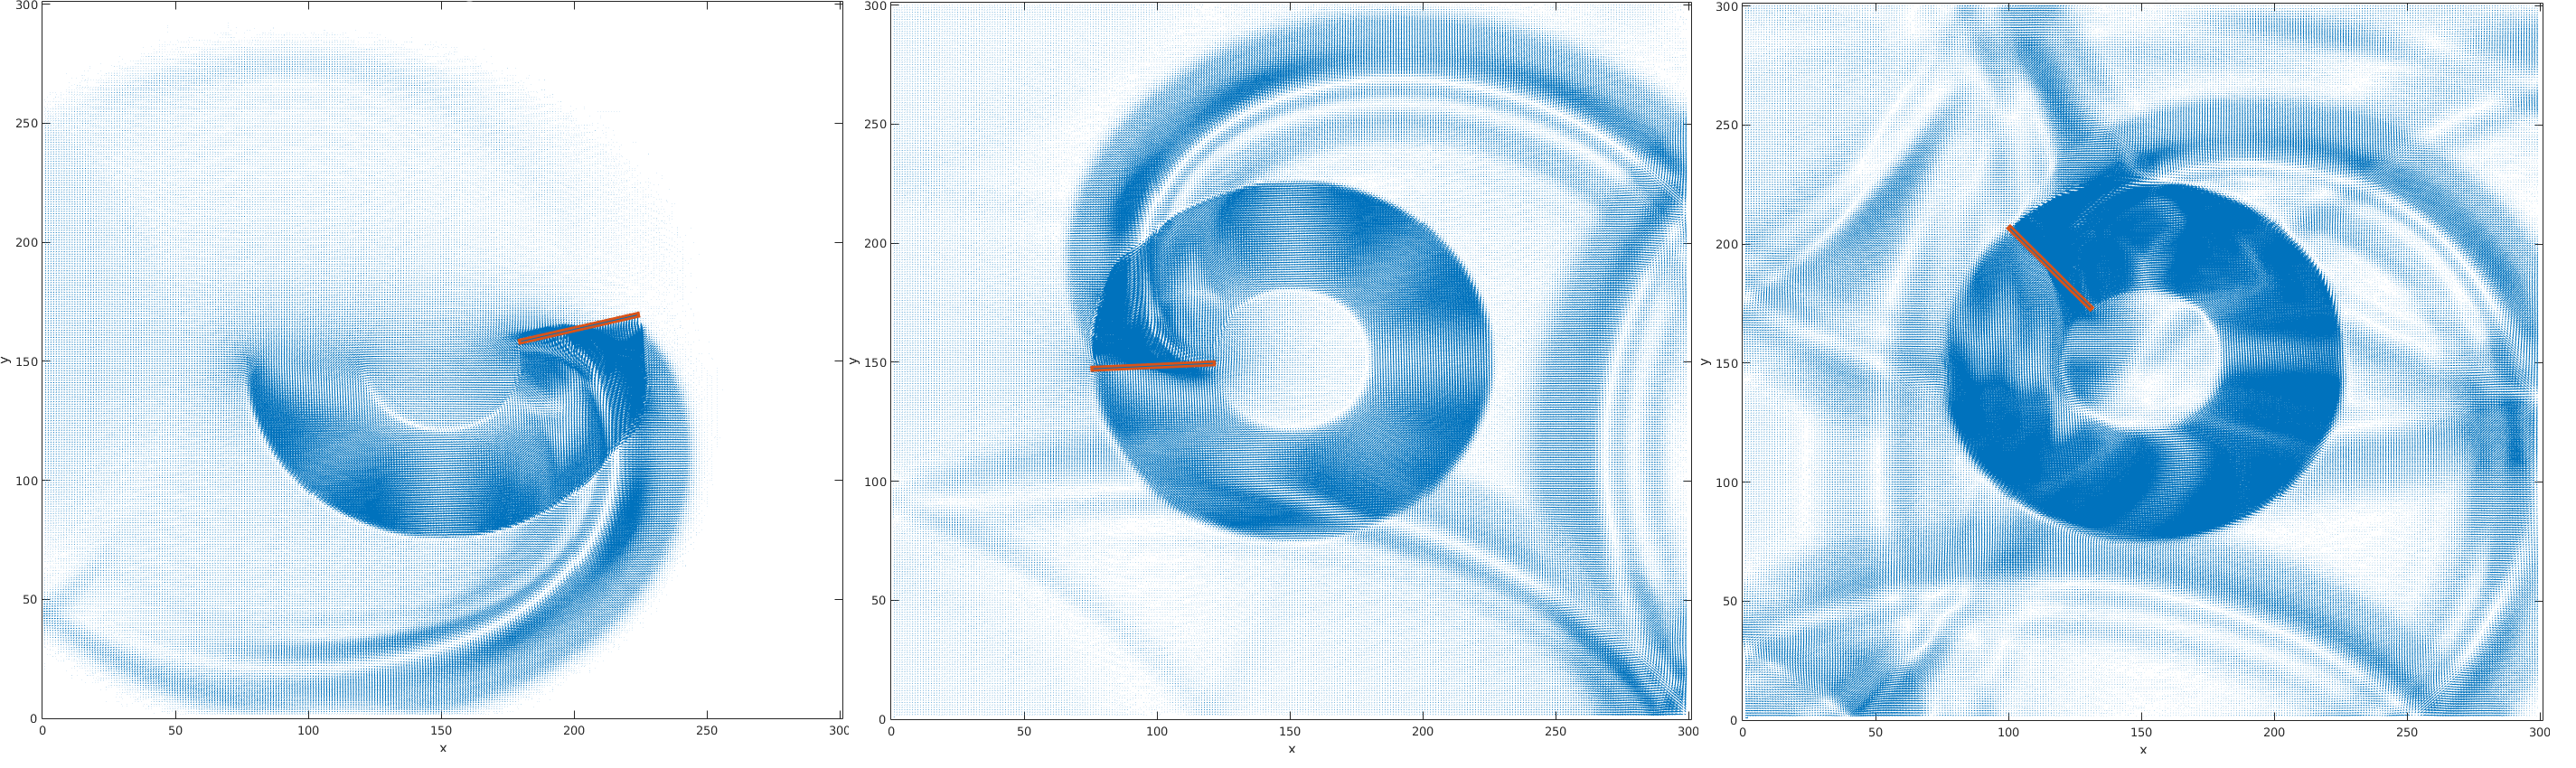
\includegraphics[width=\textwidth,height=4cm]{figures/sim_vf_all}
\caption{El aspa (rojo) empuja al fluido al rotar.}
\label{fig:sim_vf_all}
\end{figure*}

Se aprecia claramente la posición del aspa rotante que empuja el fluido, así como las ondas producidas por este movimiento. Las mismas reflejan correctamente en la pared del contenedor, y la dirección de rotación obtenida es la esperada por el empuje de un aspa moviéndose en esa dirección.

~\\
Fueron realizados estudios de rendimiento para medir el impacto de la ejecución en paralelo. Como marco teórico de esta sección, se utilizó por un lado la Ley de Amdahl, midiendo así el speedup $S(n,p) = \frac{T_{ser}(n) }{ T_{par}(n,p)}$  a trabajo fijo aumentando la cantidad de procesadores, y por otro la Ley de Gustavson para la cual se midió el trabajo realizado por cantidades cada vez mas grandes de recursos de procesamiento a tiempo constante. Luego se calculó la eficiencia $E(n,p) = \frac{S(n,p)}{p}$. Donde $ T_{ser}(n)$  es el tiempo que tarda el programa en su versión serial para una entrada de tamaño n, y $T_{par}(n,p)$  es el tiempo que tarda el programa paralelo para una entrada de tamaño n y cantidad de procesos p.

\begin{subsection}{Ley de Amdahl}
~\\
La Ley de Amdahl da el speedup teórico en la ejecución de una tarea que consta de una cantidad de trabajo fijo al incrementar los recursos del sistema.
~\\
~\\
Llevada al limite, sirve para calcular la mejora máxima posible para una tarea que consta de una parte paralelizable, y una parte serial que no puede ser efectivamente paralelizada.
~\\
La formulación matemática de la Ley de Amdahl es la siguiente:
~\\
~\\
\begin{center}
$S(s) \leq  \frac{1}{(1-p)+\frac{p}{s}}$
\end{center}
~\\
~\\
Donde S es el speedup total, s el speedup de la parte del programa que se favorece por el paralelismo, y p es la proporción de tiempo que era ocupada por la parte del programa que tiene speedup alguno. Se asume que todo el tiempo que no corresponde a p, o sea 1-p, se mantiene igual. Un resultado directo de esta ley es que incluso utilizando infinitos recursos, no puede aumentarse el speedup mas que:
~\\
\begin{center}

$S(s) \leq  \frac{1}{1-p}$
\end{center}

~\\

Para este experimento se quiere dejar fija la cantidad de trabajo total realizado, y medir como cambia la velocidad al agregar unidades de procesamiento. 
~\\
~\\
El programa se ejecutó en una red ethernet con 21 maquinas, cada una disponiendo de 4 núcleos. Al momento de realizar la experimentación, estas maquinas estaban siendo utilizadas, a razón de dos nucleos por maquina, con lo cual se disponía de 42 núcleos para procesar la prueba. Los speedups resultado son los siguientes:
~\\

\begin{center}
\begin{table}[h]

    \begin{tabular}{ | l | l |}
    \hline
    CPUs & S(n,p) \\ \hline
	30 &  19.8541013255	\\ \hline
	25 &  19.2648777129	\\ \hline
	20 &  17.4229950177	\\ \hline
	15 &  15.4322650675	\\ \hline
	12 &  12.3897738475	\\ \hline
	10 &  10.5198631716	\\ \hline
	9  &  9.1780910351	\\ \hline
	8  &  8.434695922	\\ \hline
	6  &  6.0758387804	\\ \hline
	5  &  5.0493848725	\\ \hline
	3  &  2.5275473744	\\ \hline
	1  &  1	\\ \hline
    \end{tabular}
    \caption{Los datos de esta tabla pueden ser apreciados en la figura \ref{fig:exp_amdahl_speedup}}
\end{table}
\end{center}

\begin{figure}
\textbf{Speedup}\par\medskip

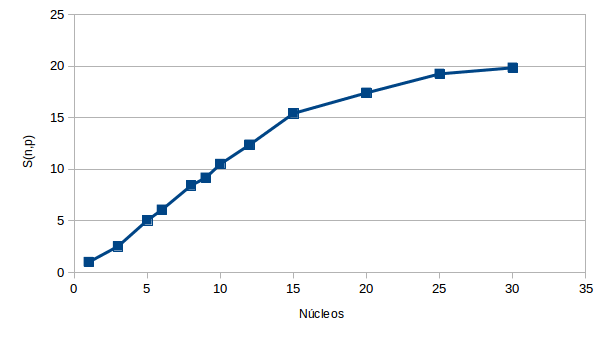
\includegraphics[width=.75\textwidth,height=.75\textheight,keepaspectratio]{figures/exp_amdahl_speedup}
\caption{El speedup tiende a disminuir al aumentar mucho la cantidad de nucleos, perdiendo aproximadamente un tercio del rendimiento al alcanzar los 30.}
\label{fig:exp_amdahl_speedup}

\end{figure}

\end{subsection}


\begin{subsection}{Ley de Gustavson}
~\\
La Ley de Gustavson calcula el speedup teórico para una tarea de tiempo de ejecución fijo al incrementar los recursos de un sistema. Al aplicar la Ley de Gustavson, lo que varia no es el tiempo de ejecución, sino la cantidad de trabajo realizado. La formulación matemática de la Ley de Gustavson es la siguiente:
~\\
{\centering
$S(s) = p - \alpha(p-1)$
}
~\\
Donde S es el speedup, p es el número de procesadores, y $\alpha$ la parte no paralelizable del proceso. Notar que si se aumenta notablemente la el trabajo total en la sección paralelizable, haciendo que la proporción de trabajo serial $\alpha$ sea muy pequeña, esto resulta en algo muy similar a $S(s) = p$
~\\
Según Gustavson, en su trabajo de 1988, tiene mucho mas sentido hablar de tiempo fijo que de tamaño fijo. Esto es así porque en la practica los tiempos utilizados para realizar simulaciones no varían tanto como los tamaños o cantidad de recursos utilizados para las mismas. Siguiendo este espíritu, en este experimento se fija el tiempo limite en 120s, y se mide cuanta utilidad, o trabajo neto, pudo extraerse para distintas cantidades de unidades de procesamiento.
~\\
Para lograr esto, programa fue nuevamente ejecutado en una red ethernet con 21 maquinas, cada una disponiendo de 3 núcleos. Al momento de realizar la experimentación, estas maquinas estaban siendo utilizadas, a razón de un núcleo por maquina, con lo cual se disponía de 63 núcleos para procesar la prueba. 
~\\
~\\
Como medida de trabajo efectivo, se contó la cantidad de elementos del sistema calculados, ya que es lo que da utilidad. Se aclara que cuando en la tabla de resultados figura que se utilizó un solo núcleo, esa medición fue realizada sobre la versión serial del programa, no perdiendo así tiempo inicializaciónes o cálculos necesarios para paralelizar. Los resultados son los siguientes, que también pueden apreciarse en la figura \ref{fig:exp_gustafson_work}. También se calcula el trabajo normalizado por núcleo, obteniéndose así los datos que se ven en la figura \ref{fig:exp_gustafson_work_norm}
~\\

\begin{center}
\begin{table}[h]
    \begin{tabular}{ | l | l |}
    \hline
CPUs   & elementos calculados \\ \hline
1      & 111.113 Millones \\ \hline
5      & 413.814 Millones \\ \hline
20     & 1976.24 Millones \\ \hline
35     & 3198.04 Millones \\ \hline
50     & 3661.31 Millones \\ \hline
60     & 4294.03 Millones \\ \hline
    \end{tabular}
    \caption{Datos de la figura \ref{fig:exp_gustafson_work}}
\end{table}
\end{center}



\begin{figure}
\textbf{Trabajo}\par\medskip

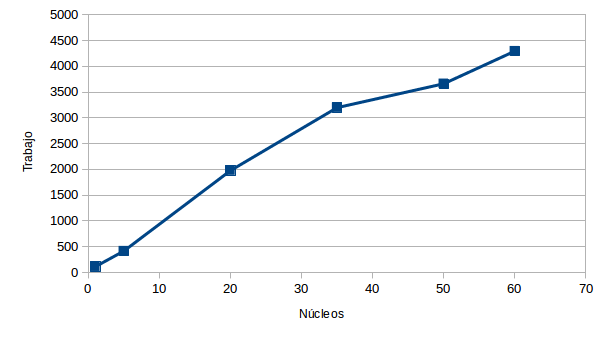
\includegraphics[width=.75\textwidth,height=.75\textheight,keepaspectratio]{figures/exp_gustafson_work}
\caption{el trabajo neto calculado se comporta de forma aproximadamente lineal.}
\label{fig:exp_gustafson_work}
\end{figure}
Los datos parecen indicar un comportamiento que escala correctamente con la cantidad de núcleos. En la siguiente tabla sin embargo, se muestra el trabajo por núcleo, y se ve que decrece con el aumento de los recursos.


\begin{center}
\begin{table}[h]
    \begin{tabular}{ | l | l |}
    \hline
CPU   & trabajo/núcleos \\ \hline
1     &  111.113 \\ \hline
5     &  82.7628 \\ \hline
20    &  98.8120 \\ \hline
35    &  91.3725 \\ \hline
50    &  73.2262 \\ \hline
60    &  71.5671 \\ \hline
    \end{tabular}
    \caption{Trabajo por nucleo. }
\end{table}
\end{center}



En particular, si normalizamos los datos respecto del trabajo realizado por la versión serial, notamos una reducción del rendimiento de la simulación que llega a bajar hasta un 64\% respecto del rendimiento extraído por un solo núcleo.


\begin{center}
\begin{table}[h]
    \begin{tabular}{ | l | l |}
    \hline
CPUs & trabajo/(núcleos*111.113) \\ \hline
1    & 1 \\ \hline
5    & 0.7448 \\ \hline
20   & 0.8892 \\ \hline
35   & 0.8223 \\ \hline
50   & 0.6590 \\ \hline
60   & 0.6440 \\ \hline
    \end{tabular}
    \caption{Trabajo normalizado.}
\end{table}
\end{center}

\begin{figure}
\textbf{Trabajo normalizado}\par\medskip

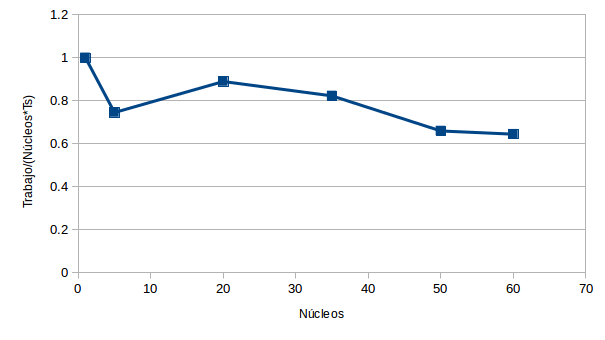
\includegraphics[width=.75\textwidth,height=.75\textheight,keepaspectratio]{figures/exp_gustafson_work_norm}
\caption{Al normalizar se nota mas fácilmente la desviación de la linealidad.}
\label{fig:exp_gustafson_work_norm}

\end{figure}



~\\

 A primera vista, parece que se pierde mucho rendimiento. En realidad, si tenemos en cuenta que la corrida de un solo núcleo fue realizada con una versión distinta que no incluye código de MPI, se entiende que ese valor aparezca como un outlier. Dicho esto, lo que esperaríamos ver si el programa escalara, seria una recta horizontal a partir de la segunda medición. Si bien no es el resultado obtenido, no se dista demasiado. Lo importante es que se puede aumentar la cantidad de trabajo realizable significativamente agregando unidades de procesamiento, lo cual es un resultado mas optimista que el insinuado por la Ley de Amdahl.
~\\
~\\
Otra medida importante relacionada con la ley de Gustavson, que ya fue mencionada anteriormente es la eficiencia. Con el objetivo de medirla se realizó otra experimentación en la cual varia la cantidad de nucleos y el tamaño del problema. Recordemos que la definición de eficiencia es  $E(n,p) = \frac{S(n,p)}{p}$.
~\\
Los tiempos conseguidos en esta etapa de la experimentación son los siguientes.
~\\

\begin{center}
\begin{table}[h]
    \begin{tabular}{ | l | l | l | l | l |}
    \hline
CPUs & raíz(2,n) & Tp & Ts & E(n,p) \\ \hline

80   & 100  &  105.000 & 7731.128 & 0.920 \\ \hline
40   & 75   &  74.730  & 2435.544 & 0.814 \\ \hline
20   & 50   &  61.764s & 713.772 & 0.577 \\ \hline
5    & 50   &  252.129 & 713.772 & 0.566 \\ \hline
1    & 1    &  0.366   & 0.366 & 1 \\ \hline
   \end{tabular}
    \caption{Eficiencia. }
\end{table}
\end{center}
~\\


Si vemos la figura \ref{fig:exp_gustafson_eficiency}, encontramos devuelta que si bien la eficiencia no es optima, el resultado es mucho mejor que el esperado al seguir el paradigma planteado por la ley de Amdahl. También puede verse nuevamente la diferencia entre la versión serial y la versión paralela para tareas de poco trabajo en el primer punto del gráfico.
Como nota aparte, la eficiencia es una medida mucho mas sensible de la escalabilidad que el speedup, como podemos apreciar si comparamos este ultimo gráfico, con el gráfico de speedup (figura \ref{fig:exp_gustafson_speedup}) de los mismos datos.


\begin{figure}
    \textbf{Eficiencia}\par\medskip

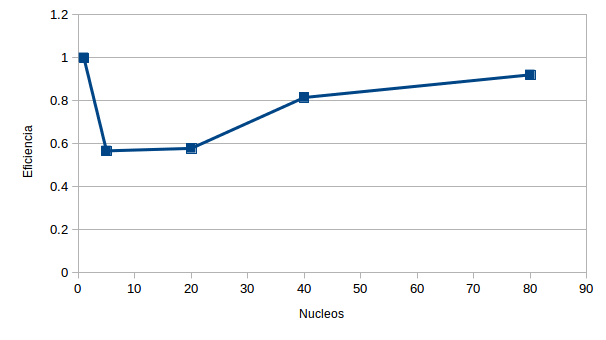
\includegraphics[width=.75\textwidth,height=.75\textheight,keepaspectratio]{figures/exp_gustafson_eficiency}
\caption{La eficiencia esta normalizada en función de la cantidad de núcleos, por lo que es muy sensible a las desviaciones de la linealidad.}
\label{fig:exp_gustafson_eficiency}
\end{figure}


\begin{figure}
\textbf{Speedup}\par\medskip
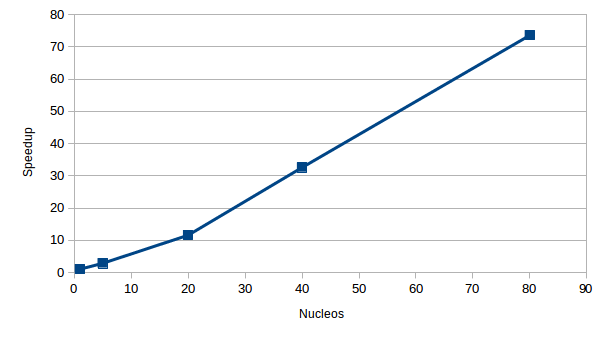
\includegraphics[width=.75\textwidth,height=.75\textheight,keepaspectratio]{figures/exp_gustafson_speedup}
\caption{Al graficar el speedup, se nota mucho menos el comportamiento no lineal.}
\label{fig:exp_gustafson_speedup}
\end{figure}

\end{subsection}
\end{section}
